\documentclass[conference]{IEEEtran}

\usepackage{etoolbox}

\renewcommand{\IEEEbibitemsep}{7pt}

\patchcmd{\thebibliography}
  {\footnotesize}
  {\small}
  {}
  {}
\renewcommand{\refname}{\normalsize REFERENCES}
\IEEEoverridecommandlockouts
\usepackage{cite}
\usepackage{amsmath,amssymb,amsfonts}
\usepackage{algorithmic}
\usepackage{algorithm}
\usepackage{graphicx}
\usepackage{textcomp}
\usepackage{xcolor}
\usepackage{booktabs}
\usepackage{multirow}
\usepackage{url}
\usepackage[hidelinks]{hyperref}
\usepackage{tikz}
\usetikzlibrary{positioning,arrows.meta}

%% Custom Card Suit Symbols
\newcommand{\spades}{\spadesuit}
\newcommand{\hearts}{\textcolor{red}{\heartsuit}}
\newcommand{\diamonds}{\textcolor{red}{\diamondsuit}}
\newcommand{\clubs}{\clubsuit}



\def\BibTeX{{\rm B\kern-.05em{\sc i\kern-.025em b}\kern-.08em
    T\kern-.1667em\lower.7ex\hbox{E}\kern-.125emX}}

\newcommand*{\affaddr}[1]{#1} 
\newcommand*{\affmark}[1][*]{\textsuperscript{#1}}
\newcommand*{\email}[1]{\texttt{#1}}

\begin{document}

%% ============================================================
%% TITLE
%% ============================================================
\title{PANES : Policy-guided Asymmetric Nash Equilibrium Search}

\author{
\IEEEauthorblockN{Youhan lalwani}
\IEEEauthorblockA{\textit{Department of Artificial Intelligence} \\
\textit{and Data Science}\\
\textit{Thadomal Shahani Engineering}\\
\textit{College}\\
\textit{Mumbai, India} \\
\underline{\textcolor{blue}{youhanlalwani@gmail.com}}}
\and
\IEEEauthorblockN{Mahesh Patel}
\IEEEauthorblockA{\textit{Department of Artificial Intelligence} \\
\textit{and Data Science}\\
\textit{Thadomal Shahani Engineering}\\
\textit{College}\\
\textit{Mumbai, India} \\
\underline{\textcolor{blue}{patelbhiyaram757@gmail.com}} \\[-1.2em]
\phantom{\underline{\textcolor{blue}{}}}}
\and
\IEEEauthorblockN{Parthavi Gaikwad}
\IEEEauthorblockA{\textit{Department of Artificial Intelligence} \\
\textit{and Data Science}\\
\textit{Thadomal Shahani Engineering}\\
\textit{College}\\
\textit{Mumbai, India} \\
\underline{\textcolor{blue}{pgaikwad0601@gmail.com}}}
\and
\IEEEauthorblockN{\hspace*{1.7em}Astha Mishra}
\IEEEauthorblockA{\hspace*{1.5em}\textit{Department of Artificial Intelligence} \\
\hspace*{1.5em}\textit{and Data Science}\\
\hspace*{1.5em}\textit{Thadomal Shahani Engineering}\\
\hspace*{1.5em}\textit{College}\\
\hspace*{1.5em}\textit{Mumbai, India} \\
\hspace*{1.5em}\underline{\textcolor{blue}{asthamishra1905@gmail.com}} \\[-1.2em]
\phantom{\underline{\textcolor{blue}{}}}}
\and
\IEEEauthorblockN{\hspace*{1.5em}Dr. Sanober Shaikh}
\IEEEauthorblockA{\hspace*{1.5em}\textit{Department of Artificial Intelligence} \\
\hspace*{1.5em}\textit{and Data Science}\\
\hspace*{1.5em}\textit{Thadomal Shahani Engineering}\\
\hspace*{1.5em}\textit{College}\\
\hspace*{1.5em}\textit{Mumbai, India} \\
\hspace*{1.5em}\underline{\textcolor{blue}{sanober.shaikh@thadomal.org}} \\[-1.2em]
\hspace*{1.5em}\underline{\textcolor{blue}{}}}
\and
\IEEEauthorblockN{\phantom{}}
\IEEEauthorblockA{\phantom{\textit{Department of Artificial Intelligence}} \\
\phantom{\textit{and Data Science}}\\
\phantom{\textit{Thadomal Shahani Engineering}}\\
\phantom{\textit{College}}\\
\phantom{\textit{Mumbai, India}} \\
\phantom{\underline{\textcolor{blue}{}}}}
}

\maketitle

%% ============================================================
%% ABSTRACT
%% ============================================================
\begin{abstract}
Trick-taking card games with mandatory bidding confront reinforcement learning agents with a distinctive two-phase problem: each player must commit to a numeric bid before any cards are played, and whether that bid turns out to be correct hinges on adversarial interactions unfolding over many subsequent tricks. Judgement (also called Oh~Hell) makes this harder still through its Hook rule, which structurally prevents the total bids from summing to the available tricks. This ensures at least one player is guaranteed to fail every round. Here, we introduce a complete framework of reinforcement learning for the Judgement game, consisting of an environment and a specific agent architecture trained together in bidding and trick-play under imperfect information. The environment was built inside the RLCard platform, supporting four-player games with legal-action masking and lightweight state rollback for tree search. On top of this, we developed a PANES agent that pairs Neural Fictitious Self-Play with Information Set Monte Carlo Tree Search. During training, the agent learns through self-play guided by dense trick-level reward shaping; at decision time, it runs multi-step lookahead over determinized game worlds using the learned opponent policies. In a 2{,}000-game paired-deal arena evaluation, the PANES agent reached $22.7\%$ bid accuracy versus $13.5\%$ for the neural-only baseline---a $68\%$ relative gain, supported by robust statistical significance ($p < 0.0001$). A closer look at the training dynamics revealed an interesting asymmetry: agents pick up trick-winning skills quickly but struggle much more with deliberate trick avoidance, which we identify as the main learning bottleneck. We also ran an ablation with Prioritized Experience Replay; it cut training loss by roughly a third yet produced no measurable improvement in game-level performance, pointing to the credit assignment horizon as the binding constraint. Taken together, these findings show that merging equilibrium-based self-play with online tree search is a viable path for imperfect-information trick-taking games, while the long-horizon credit assignment problem remains the central open challenge.
\end{abstract}

\begin{IEEEkeywords}
Reinforcement Learning, Monte Carlo Tree Search, Neural Fictitious Self-Play, Imperfect-Information Games, Trick-Taking Card Games, Nash Equilibrium, Multi-Agent Systems, Dense Reward Shaping
\end{IEEEkeywords}

%% ============================================================
%% I. INTRODUCTION
%% ============================================================
\section{\large \textbf{Introduction}}
Reinforcement learning has come a long way in game playing, but partially observable environments (which have game players with private information) are inherently harder to solve. Card games are a prime example: each hand is private, there's long horizons between actions, and the optimal move depends on the other player's hidden state. Although deep RL has been successful for other trick-based card games, e.g., DouZero~\cite{zha2021douzero}, PerfectDou~\cite{you2020perfectdou}, these programs are either game-specific or require the oracle teaching of the current trick. Other trick-taking card games that include forced bidding is largely uncharted territory.


Judgement (also called Oh\~Hell) is an example. After players have bid how many tricks they think they will win, players will proceed with an adversarial game of 13 tricks, playing cards back and forth between them. The unique Hook rule prevents the dealer from bidding just that many tricks to the total sum of tricks players believe they will win, creating a game where someone will always lose. Equally important, overbidding and underbidding carry the same penalty, forcing agents to learn not just how to win tricks but also when to deliberately lose them.

Judgement is difficult for standard RL due to 52 actions seperating the first action and terminal eeward~\cite{sutton2018reinforcement}. NFSP~\cite{silver2016deep} learns equilibrium strategies but only looks 1 step ahead, while MCTS~\cite{browne2012survey} looks ahead but doesnt rely on learned knowledge. 

We address both gaps by extending NFSP self-play with extensive reward shaping and void-aware determinization, building on the work of Zhang et al.~\cite{zhang2021mcnfsp} and propose \textbf{PANES} (Policy-guided Asymmetric Nash Equilibrium Search) for trick-taking card games. Our contributions are : 

\begin{enumerate}
    \item A complete Judgement environment within RLCard~\cite{zha2021rlcard}, with a 454-dimensional state space, 66-action discrete space, and lightweight checkpoint support for tree search.
    \item A dense reward framework for the 13-trick credit assignment problem, providing trick-level bid-alignment signals on top of the sparse terminal score.
    \item The PANES agent: asymmetric IS-MCTS with MRV void-respecting determinization,and NFSP-guided opponent simulation.
    \item An empirical evaluation showing $22.7\%$ bid accuracy for PANES vs.\ $13.5\%$ for the pure neural baseline---a $68\%$ relative gain---over 2{,}000 paired-deal games ($p < 0.0001$).
\end{enumerate}

%% ============================================================
%% II. RELATED WORK
%% ============================================================
\section{\large \textbf{Related Work}}
There are two types of algorithms we can use to address sequential imperfect information decision-making: equilibrium-finding algorithms and online search. Fictitious play~\cite{brown1951iterative, robinson1951} and its deep counterpart, Neural Fictitious Self-Play (NFSP)~\cite{silver2016deep}, learn to approximate Nash equilibria in large games via an combination of a best-response DQN~\cite{mnih2015human} and a supervised average policy network. NFSP can avoid cycle exploitation, but the one-step TD backups used in NFSP makes the learned equilibria` unsuitable for long-horizon tasks. 

Conversely, Information Set Monte Carlo Tree Search (ISMCTS)~\cite{browne2012survey, cowling2012ismcts} learns strong multi-step lookahead strategies for games by building search trees over determinized states of the game. It is limited, however, by building a new search tree for each decision, it suffers from strategy fusion~\cite{frank1998search} in high-uncertainty state spaces, and it does not learn to transfer strategic knowledge across games.

To address this shortcoming, Zhang et al.~\cite{zhang2021mcnfsp} later proposed MC-NFSP, with the single-step Q-value estimate replaced by MCTS rolls under the evaluation of average policy. While this results in a strong two-player poker system, transitioning search-learning integration to multi-player trick-taking games such as Judgement introduces distinct challenges: 1) opponent behavior must be well simulated under forced following rules, requiring void-aware determinization, 2) search trees expand exponentially with the number of players.  In-context opponent modeling~\cite{opponentmodeling2024} suggests it could be beneficial but it comes at a significant inference overhead. Our proposed PANES tackles these issues through an asymmetric tree search where the opponents are modeled by learned policies.

Propagating reward signals over long trick sequences is another major challenge. Potential-based reward shaping~\cite{ng1999policy} guarantees policy invariance but it requires hand-crafted potential functions. Alternative methods like Prioritized Experience Replay (PER)~\cite{schaul2016prioritized} prioritize informative states but do not shorten the horizon. Algorithms such as DouZero~\cite{zha2021douzero} and PerfectDou~\cite{you2020perfectdou} use Monte Carlo returns or oracle-guided value networks to handle sparse signals, but they either suffer from high variance or require parallel training of privileged models. In contrast, our dense trick-level schedule guides bidding and play alignment dynamically without auxiliary networks. Finally, while platforms like RLCard~\cite{zha2021rlcard} and OpenSpiel~\cite{lanctot2019openspiel} standardize card game evaluation, neither supports the multi-stage bidding and play dynamics of Judgement, a gap our environment fills.

%% ============================================================
%% III. ENVIRONMENT DESIGN
%% ============================================================
\section{\large \textbf{The Judgement Game Environment}}
 
Building an RL environment for Judgement means turning the informal rules of a card game into a precisely specified decision process -- without losing the structural properties that make the game strategically interesting. We kept three design principles in mind throughout: (1) all publicly available information should be fully observable, with private hands properly masked; (2) rule enforcement should live entirely inside the environment, with no game-rule knowledge leaking into agent code; and (3) game-state serialization must be efficient enough to support the many rollbacks required by MCTS. The resulting implementation is integrated into the RLCard framework~\cite{zha2021rlcard}, making it the first trick-taking game supported by that platform.
 
\subsection{\textbf{Formal Problem Formulation}}
 
We define Judgement as a four-player imperfect information extensive-form game, following the Markov game framework~\cite{Littman1994MarkovGA}. The decision problem faced by each player is modeled as a Partially Observable Markov Decision Process (POMDP) defined by the tuple $\langle \mathcal{S}, \mathcal{O}, \mathcal{A}, \mathcal{T}, \mathcal{R}, \gamma, \mathcal{P}_0 \rangle$. Here, $\mathcal{S}$ represents the set of all possible world states (deck distribution, private hands, bids, trick history); $\mathcal{O} \subset [0,1]^{454}$ is the local observation space of each player, masking private opponent hands; $\mathcal{A}$ is the $66$-dimensional action space with a legal-action mask; $\mathcal{T}$ represents transition dynamics; $\mathcal{R}$ is the reward function; $\gamma=0.995$ is the discount factor; and $\mathcal{P}_0$ is the initial uniform dealing distribution. The training objective is to find a joint policy profile $\boldsymbol{\pi}=(\pi_1,\dots,\pi_4)$ approaching a Nash equilibrium via Neural Fictitious Self-Play~\cite{silver2016deep}.
 
\begin{table}[htbp]
\centering
\caption{\normalsize Observation Space Decomposition (454 Features)}
\label{tab:obsspace}
\scalebox{0.95}{
\small
\begin{tabular}{@{}lcl@{}}
\toprule
\textbf{Component} & \textbf{Dim.} & \textbf{Encoding} \\
\midrule
Player's Hand & $52$ & Multi-hot bitmask \\
Trump Suit & $4$ & One-hot indicator \\
Agent's Own Bid & $14$ & One-hot ($0$--$13$) \\
Other Players' Bids & $3\times14=42$ & One-hot per player \\
Tricks Won (all players) & $4\times14=56$ & One-hot per player \\
Current Trick Cards & $4\times52=208$ & Per-seat card slot \\
Played Cards History & $52$ & Cumulative multi-hot \\
Round Card Count & $14$ & One-hot ($1$--$13$) \\
Phase Indicator & $1$ & Binary (bid/play) \\
Current Player & $4$ & One-hot indicator \\
Round Progress & $1$ & Fraction $\text{round\_idx}/\text{total}$ \\
Hand Strength Heuristics & $6$ & Continuous $[0,1]$ \\
\midrule
\textbf{Total} & \textbf{454} & \\
\bottomrule
\end{tabular}
}
\end{table}
 
\subsection{\textbf{Game Rules and Action Space}}
 
Judgement is a $52$-card game for four players. In our training setup we fix hand size to $n=13$ tricks, with the trump suit rotating deterministically ($\spadesuit \rightarrow \diamondsuit \rightarrow \clubsuit \rightarrow \heartsuit$) each round to prevent overfitting. Each round has two phases: (1) \textit{Bidding Phase} (Actions $0$--$13$): players sequentially declare a predicted trick count $b_i \in \{0,\dots,n\}$, with the dealer bidding last under the Hook constraint ($\sum b_i \neq n$), guaranteeing that at least one player fails to meet their contract. (2) \textit{Playing Phase} (Actions $14$--$65$): the player to the dealer's left leads the first trick; subsequent players must follow suit if able, otherwise discarding or trumping, and the trick is won by the highest card of the led suit or the highest trump played. The action space consists of $66$ distinct actions spanning these two phases. The environment provides a legal-action mask at every step to enforce the rules.
 
Instead of using the standard trick-scoring convention $\pm$($10+b_i$), which incentivizes bid inflation, we use a binary scoring system:
\begin{equation}
    r_i =
    \begin{cases}
        +1.0 & \text{if } w_i = b_i, \\
        -1.0 & \text{if } w_i \neq b_i,
    \end{cases}
    \label{eq:binary_score}
\end{equation}
where $w_i$ is the number of tricks won.
 
The game state is encoded as a $454$-dimensional vector of values in $[0,1]$ to bound gradient norms, detailed in Table~\ref{tab:obsspace}. Cards are mapped to $\{0,\dots,51\}$ via $\text{suit}\times13+\text{rank}$. Instead of a flat history, we use four separate $52$-bit fields to track which player played each card in the current trick, preserving temporal and seating correlations. To accelerate early learning, we append $6$ hand-strength features representing the ratio, high-card count, and average rank of trump and non-trump suits in the agent's hand.
 
%% ============================================================
%% IV. METHODOLOGY
%% ============================================================
\section{\large \textbf{Methodology}}
 
Our approach unfolds in two stages. We first train a population of NFSP agents purely through self-play, which leaves each of the four players with both a best-response Q-network and an average-policy network. Once training has converged, we wrap every trained agent in a PANES shell that runs Information Set MCTS at inference time, using the learned policies to simulate opponents and to score leaf states during search.
 
\subsection{\textbf{NFSP Training Architecture}}
 
Each player runs an independent NFSP agent~\cite{silver2016deep}, and all four share the same multilayer perceptron:
\begin{equation}
    \text{Linear}(454) \rightarrow 1024 \rightarrow 512 \rightarrow 256 \rightarrow 66
    \label{eq:network}
\end{equation}
with ReLU activations, trained with Adam~\cite{kingma2015adam} at a learning rate of $5\times10^{-4}$: the Q-network against MSE loss over bootstrapped targets, the average-policy network against NLL loss over supervised action distributions. Agents act through an anticipatory mixing strategy -- greedy best response with probability $\eta=0.15$, the average policy otherwise -- which keeps the population from cycling into exploitable patterns during multiplayer self-play. The Q-network itself follows a Double DQN scheme with target refreshes every $500$ steps and $\varepsilon$-greedy exploration decayed from $1.0$ to $0.1$ over $2.1\times10^6$ steps, drawing batches of $512$ from a $350{,}000$-capacity replay buffer, while the average-policy network trains on a reservoir buffer of the same size to preserve a representative record of past play.
 
\subsection{\textbf{Dense Reward Shaping}}
\label{sec:dense}
 
Credit assignment over a 13-trick, 52-action horizon is unstable under the sparse terminal payoff ($\pm1.0$) alone, so we layer two dense signals on top of it. During bidding, a hand-strength heuristic estimates the expected trick count $\hat{T}$ from the hand's ranks and trump distribution, and the agent is rewarded for bidding close to that estimate:
\begin{equation}
    r_{\text{bid}} = \max\!\left(-1.0,\;0.5-0.3|b-\hat{T}|\right).
    \label{eq:bid_reward}
\end{equation}
During play, each resolved trick is scored by whether it moves the agent's running trick count closer to or further from its bid -- rewarding trick wins while a bid is still outstanding and ducks once it is met, and penalizing the reverse, with a heavier penalty for overshooting than for falling short, since over-winning is the harder failure mode to unlearn. These per-trick scores accumulate into a running total $D_t^{(i)}$, so the reward on any transition is simply $r_t = D_{t+1}^{(i)} - D_t^{(i)}$, with the binary terminal payoff folded in at the last step. The result is one continuous target that blends trick-by-trick feedback with the true game outcome, rather than asking the agent to learn everything from a single payoff thirteen tricks later.
 
\subsection{\textbf{PANES Agent}}
\label{sec:hybrid}
 
\begin{figure*}[!t]
\centering
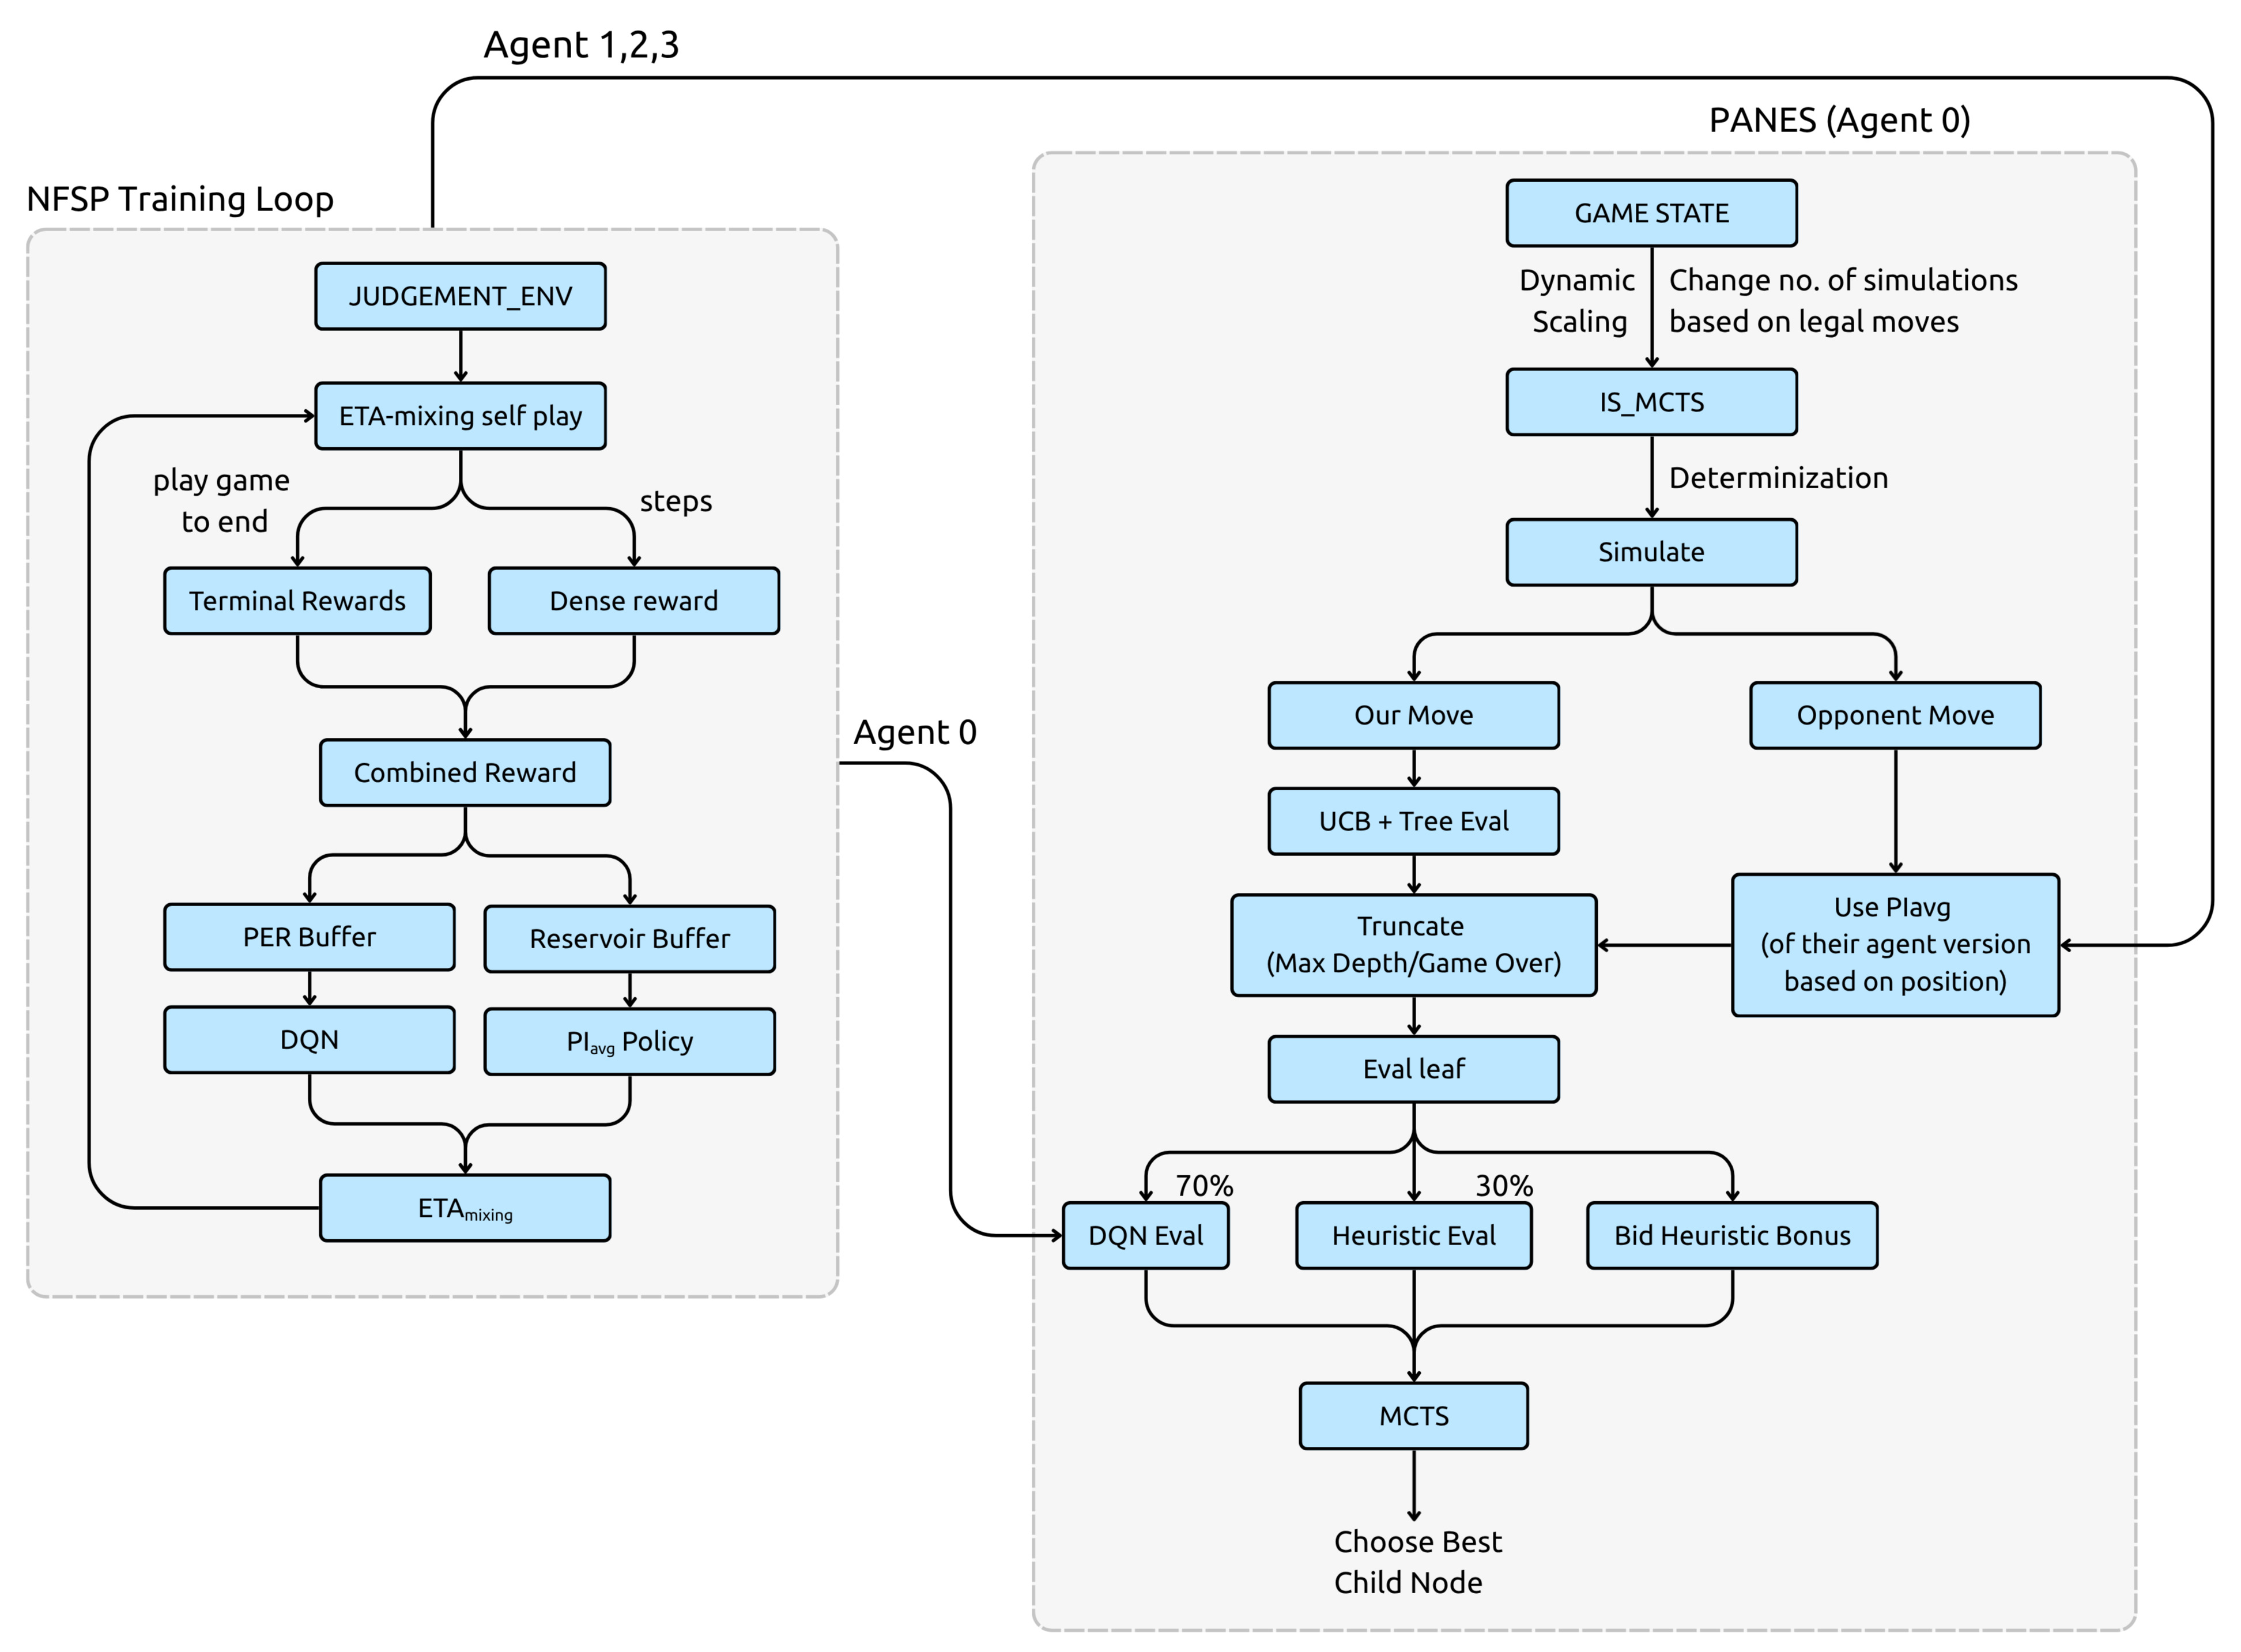
\includegraphics[width=\linewidth]{Architecture.jpeg}
\caption{The PANES architecture. Left: autonomous self-play populates the replay buffer for Q-network updates and the reservoir buffer for average-policy updates. Right: at inference, the trained networks guide Information Set MCTS as both an opponent-move simulator and a leaf-evaluation heuristic.}
\label{fig:hybrid_arch}
\end{figure*}
 
At inference time, each trained agent runs Information Set MCTS over determinized game states (Fig.~\ref{fig:hybrid_arch}). Since opponent hands are hidden, every simulation first reconstructs a plausible deal: known cards (the agent's hand, exposed trump, and played tricks) are removed from the deck, suit-following failures in the trick history are used to infer void constraints, and the remaining unknown cards are dealt to opponents ordered by how constrained they are, so void rules are respected without redeals. Rather than branch the full four-player tree -- which grows combinatorially -- the search tree is asymmetric: only the agent's own actions become nodes, while opponent turns are resolved by sampling directly from their trained average-policy network $\pi_{\text{avg}}$. Node selection follows the standard UCB1 rule~\cite{kocsis2006bandit}, and search is capped at a shallow depth of $D=2$, covering two rounds of the agent's own decisions.
 
Leaf nodes are scored with a blend of the learned Q-value and a bid-alignment heuristic,
\begin{equation}
    V_{\text{leaf}} = 0.7\,Q_{\text{DQN}}(s) + 0.3\,H_{\text{bid}}(s),
    \label{eq:leaf}
\end{equation}
where, letting $g=b_i-w_i$ be the tricks still needed and $k$ the tricks remaining,
\begin{equation}
H_{\text{bid}}(s)=
\begin{cases}
0.3+0.4(1-k/n), & g=0\ \text{(bid met)},\\[2pt]
0.1(1-g/k), & g>0,\ k\geq g,\\[2pt]
-0.5, & g>0,\ k<g\ \text{(impossible)},\\[2pt]
\text{clip}(-0.3|g|,-1,0), & g<0\ \text{(exceeded bid)}.
\end{cases}
\label{eq:hbid}
\end{equation}
This steers the search toward the exact contract while terminal states still fall back on the official binary score. Finally, because a narrow set of legal actions carries more determinization noise, the simulation budget scales up dynamically in those cases -- up to $4\times$ the base budget of $N_{\text{sim}}=200$ when three or fewer actions are legal -- so search effort concentrates where uncertainty is highest. Algorithm~\ref{alg:mcnfsp} summarizes the procedure.
 
\begin{algorithm}[htbp]
\caption{PANES Decision Procedure}
\label{alg:mcnfsp}
\begin{algorithmic}[1]
\REQUIRE Observation $s$, legal actions $A(s)$, base budget $N_{\text{sim}}$, depth limit $D=2$
\ENSURE Selected action $a^*$
\STATE $N \leftarrow$ budget scaled by $|A(s)|$ \COMMENT{Section~\ref{sec:hybrid}}
\FOR{$i=1$ \TO $N$}
    \STATE $s' \leftarrow \textsc{Determinize}(s)$ \COMMENT{MRV void-respecting deal}
    \STATE Select: descend via UCB1 while $d<D$; agent turns branch, opponent turns sample $a_{\text{opp}}\sim\pi_{\text{avg}}(\cdot\mid s')$
    \STATE Expand the resulting leaf with all $a\in A(s')$
    \STATE Fast-forward remaining opponent turns via $\pi_{\text{avg}}$ until terminal or the agent's turn
    \STATE $V_{\text{leaf}} \leftarrow 0.7\,Q_{\text{DQN}}(s') + 0.3\,H_{\text{bid}}(s')$
    \STATE \textsc{Backpropagate}$(\text{clip}(V_{\text{leaf}},-1,1))$ up the tree
\ENDFOR
\RETURN $a^* \leftarrow \operatorname*{argmax}_{a\in A(s)} N(v_0\rightarrow a)$
\end{algorithmic}
\end{algorithm}
%% ============================================================
%% V. EXPERIMENTAL SETUP
%% ============================================================
\section{\large \textbf{Experimental Setup}}
 
\subsection{\textbf{Training Configuration}}
 
All four NFSP agents train from random initialization via self-play on isolated 13-card rounds for $600{,}000$ episodes with the Adam optimizer~\cite{kingma2015adam}; Table~\ref{tab:hyperparams} lists the key hyperparameters.
 
\begin{table}[htbp]
\centering
\caption{\normalsize Training Hyperparameters}
\label{tab:hyperparams}
\scalebox{0.95}{
\small
\begin{tabular}{@{}ll@{}}
\toprule
\textbf{Parameter} & \textbf{Value} \\
\midrule
Network architecture & $454\rightarrow1024\rightarrow512\rightarrow256\rightarrow66$ \\
Learning rate (both networks) & $5\times10^{-4}$ \\
Discount factor $\gamma$ & $0.995$ \\
$\varepsilon$-decay steps & $2.1\times10^{6}$ ($150{,}000$ episodes $\times$ $14$ steps) \\
Anticipatory parameter $\eta$ & $0.15$ \\
Batch size & $512$ \\
Replay buffer capacity & $350{,}000$ \\
Reservoir buffer capacity & $350{,}000$ \\
Target network update interval & $500$ steps \\
Training frequency & Every $32$ steps \\
\bottomrule
\end{tabular}
}
\end{table}
 
\subsection{\textbf{Evaluation Pipeline}}
 The agents are evaluated using a four-phase pipeline. \\
 \textit{Phase 1 -- NFSP Training} logs taken $500$ episodes.\\ 
 \textit{Phase 2 -- PANES Evaluation} evaluates four Hybrid agents with exploration disabled ($\varepsilon=0$). \\
 \textit{Phase 3 -- Pure NFSP Baseline} runs the agents deterministically ($\eta=1$). \\
 \textit{Phase 4 -- Arena (PANES vs.\ Pure)} pits a single Hybrid agent against three Pure NFSP opponents.\\
 In the last phase we utilize paired dealings. Each deal is played twice, once with the PANES Agent and once with a Pure NFSP agent to ensure that the change in win rate is isolated from positional effects and card luck.
 
\subsection{\textbf{Metrics}}
 
We track three metrics throughout: \textit{average payoff}: the mean binary terminal reward ($\pm1.0$) across evaluation games; \textit{bid accuracy}: (``Won''), underbids (``Under''), or overbids (``Over''); and \textit{training loss trajectories}: MSE for the Q-network and NLL for the average-policy network.
 

%% ============================================================
%% VI. RESULTS
%% ============================================================
\section{\large \textbf{Results}}

\subsection{\textbf{Arena Evaluation: PANES vs.\ Pure NFSP}}
\label{sec:arena}
In Phase-4 we pit a single PANES agent against three Pure NFSP opponents across 2{,}000 paired deals (500 per seat). Each deal is played twice. Once with the Hybrid in the seat and once with a Pure NFSP agent under identical card distributions to isolate the effect of MCTS lookahead from positional and card-luck variance.

\begin{table*}[!t]
\centering
\caption{\normalsize Arena Results: PANES vs.\@ Pure NFSP (2{,}000 Paired Games)}
\label{tab:arena}
\normalsize
\renewcommand{\arraystretch}{1.2}
\setlength{\tabcolsep}{12pt}
\begin{tabular}{@{}lcccc@{}}
\toprule
\textbf{Seat} & \textbf{PANES Win \%} & \textbf{Pure Win \%} & \textbf{$\Delta$ Win \%} \\
\midrule
Random Baseline & N/A & N/A & $7.7\%$ (Theoretical) \\
\midrule
Seat 0 & $26.0\%$ & $21.2\%$ & $+4.8$ pp \\
Seat 1 & $18.6\%$ & $7.8\%$  & $+10.8$ pp \\
Seat 2 & $19.4\%$ & $9.4\%$  & $+10.0$ pp \\
Seat 3 & $26.6\%$ & $15.6\%$ & $+11.0$ pp \\
\midrule
\textbf{Average} & \textbf{$22.7\%$} & \textbf{$13.5\%$} & \textbf{$+9.2$ pp} \\
\bottomrule
\end{tabular}
\end{table*}

As shown in Table~\ref{tab:arena} and Figure~\ref{fig:arena_overall}, the PANES agent achievs $22.7\%$ bid accuracy versus $13.5\%$ for Pure NFSP. This is a $+9.2$ pp ($\mathbf{68\%}$ relative) gain, placing it at $2.9\times$ the random baseline. The advantage is consistent across all seats (Figure~\ref{fig:arena_per_seat}), with the largest swing in Seat~1 ($+10.8$ pp).

\subsection{\textbf{Statistical Validation}}

McNemar analysis (Figure~\ref{fig:mcnemar}) on the 2{,}000 paired deals shows 305 Hybrid-exclusive wins versus 120 Pure-exclusive wins ($\chi^2 = 79.66$, $p < 0.0001$). A 10{,}000-resample bootstrap (Figure~\ref{fig:bootstrap}) gives a $95\%$ CI of $[+7.3\%, +11.2\%]$ confirming the advantage is not caused by card-luck variance.


\begin{figure}[!t]
\centering
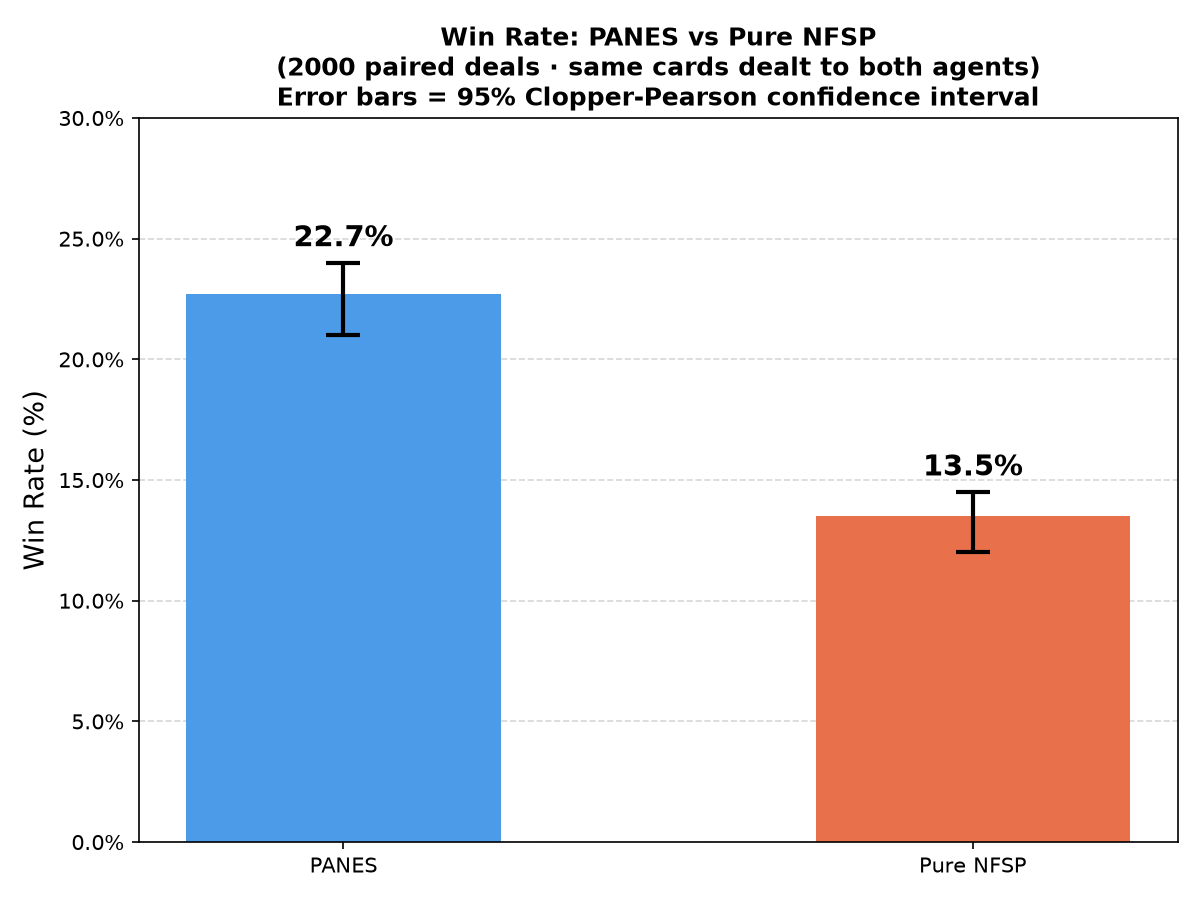
\includegraphics[width=\linewidth]{arena_overall.png}
\caption{Overall Arena Evaluation comparing 2{,}000 paired deals.}
\label{fig:arena_overall}
\end{figure}

\begin{figure}[!t]
\centering
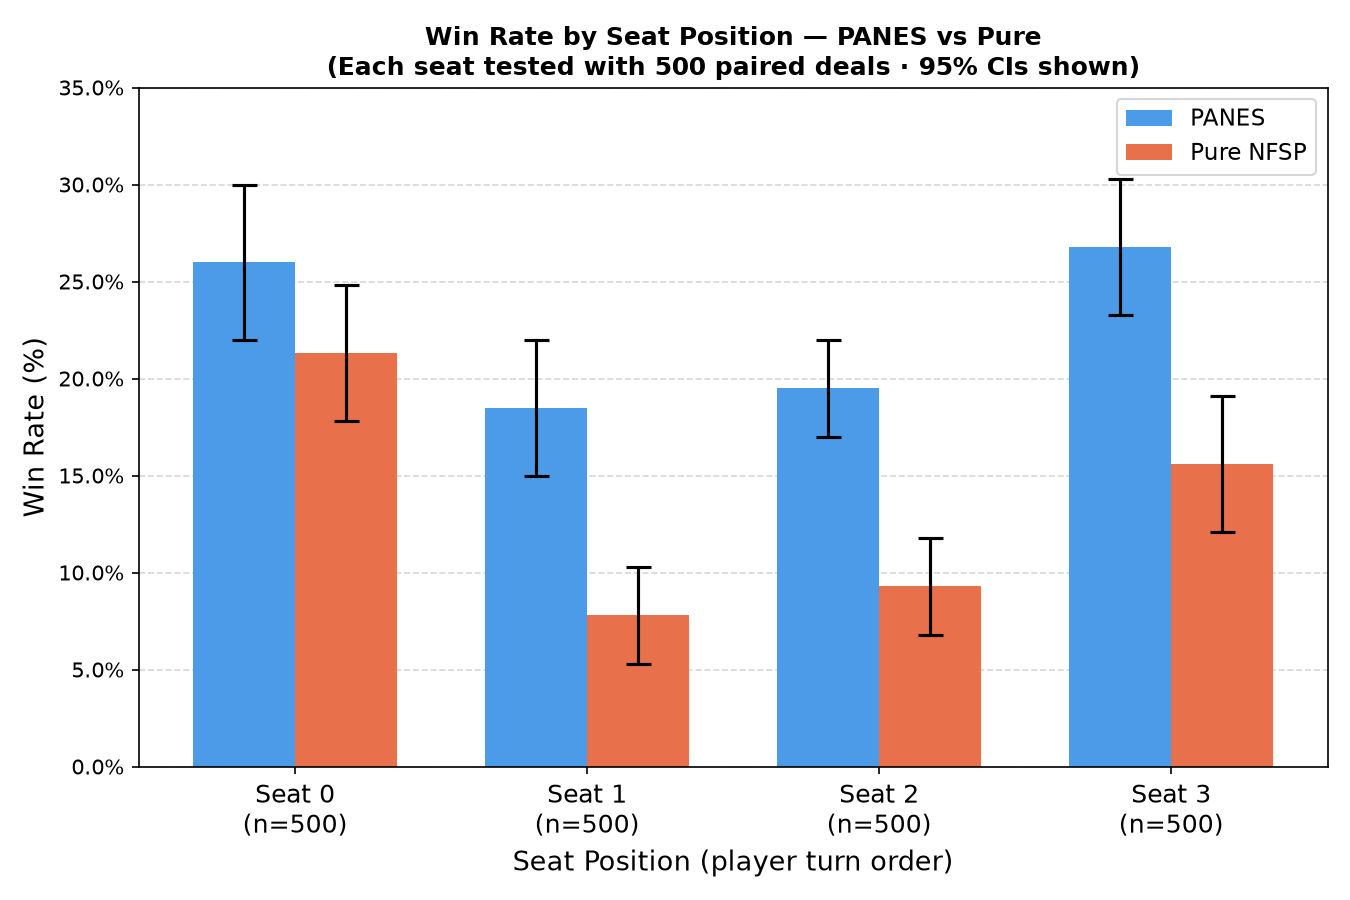
\includegraphics[width=\linewidth]{arena_per_seat.png}
\caption{Win rate grouped by starting seat position}
\label{fig:arena_per_seat}
\end{figure}

\begin{figure}[!t]
\centering
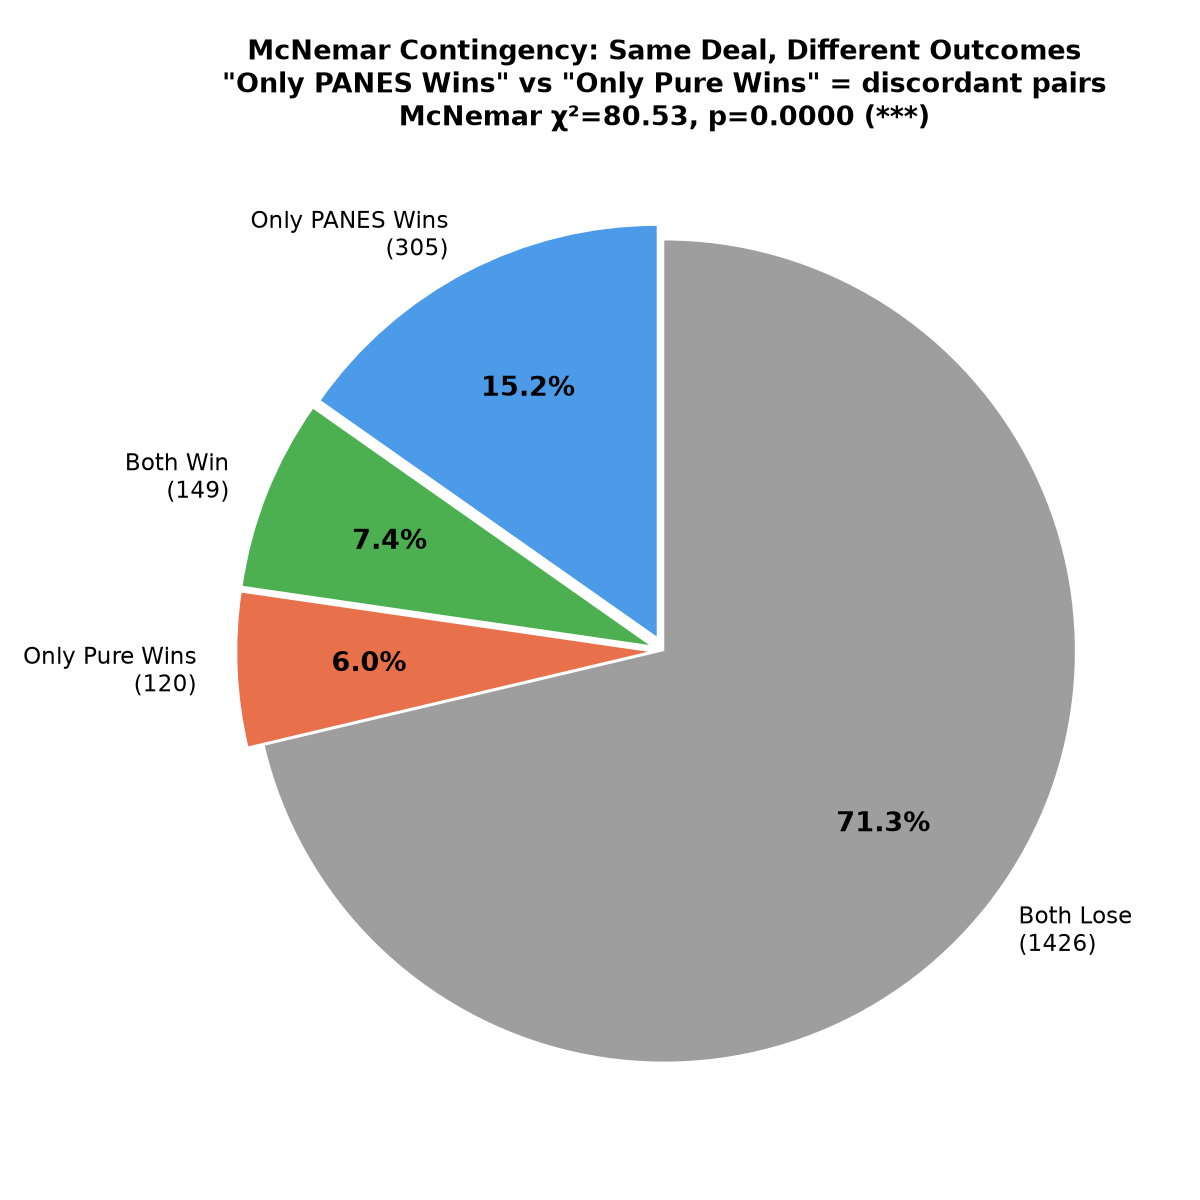
\includegraphics[width=0.85\linewidth]{mcnemar_contingency.png}
\caption{McNemar contingency breakdown highlighting discordant game pairs. The $\chi^2$ value of $79.66$ ($p < 0.0001$) indicates a significant difference in capability.}
\label{fig:mcnemar}
\end{figure}

\begin{figure}[!t]
\centering
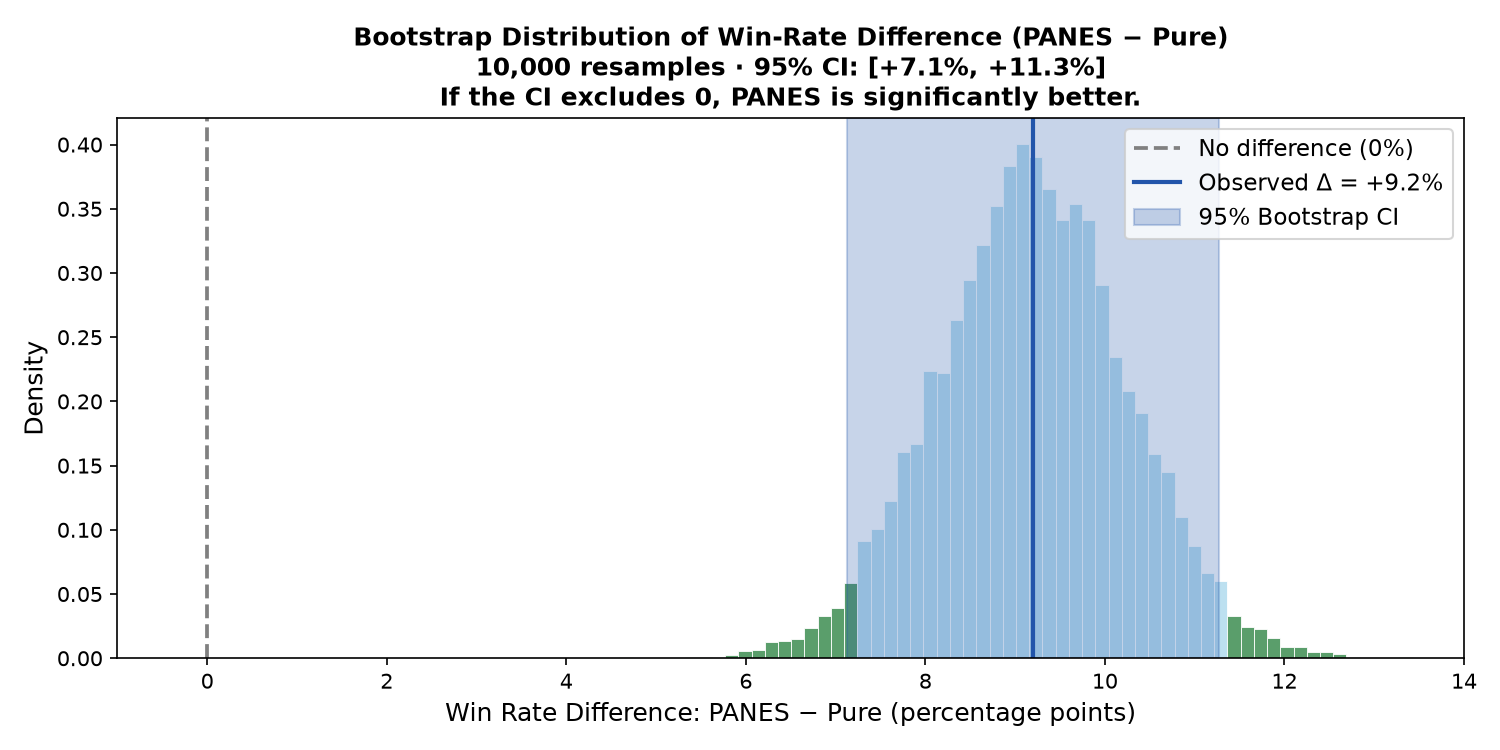
\includegraphics[width=\linewidth]{bootstrap_ci.png}
\caption{Distribution of the win-rate difference across 10{,}000 bootstrap resamples with the $95\%$ Confidence Interval highlighted.}
\label{fig:bootstrap}
\end{figure}

Training metrics are logged every 500 episodes, averaged across all seats, and smoothed with a 10{,}000-episode rolling window. The PER ablation is in Section~\ref{sec:per}.

\subsection{\textbf{Training Convergence}}

Figure~\ref{fig:training_curves} shows three training phases: an \emph{exploration phase} (0--100K) near the $7.7\%$ random baseline; a \emph{rapid learning phase} (100K--250K) where payoff climbs from $-0.84$ to $-0.79$ and accuracy reaches $\sim\!10\%$; and a \emph{plateau phase} (250K--600K) converging to $12.1\%$ accuracy---a $57\%$ improvement over random, consistent with approximate Nash equilibrium.

\begin{figure}[!t]
\centering
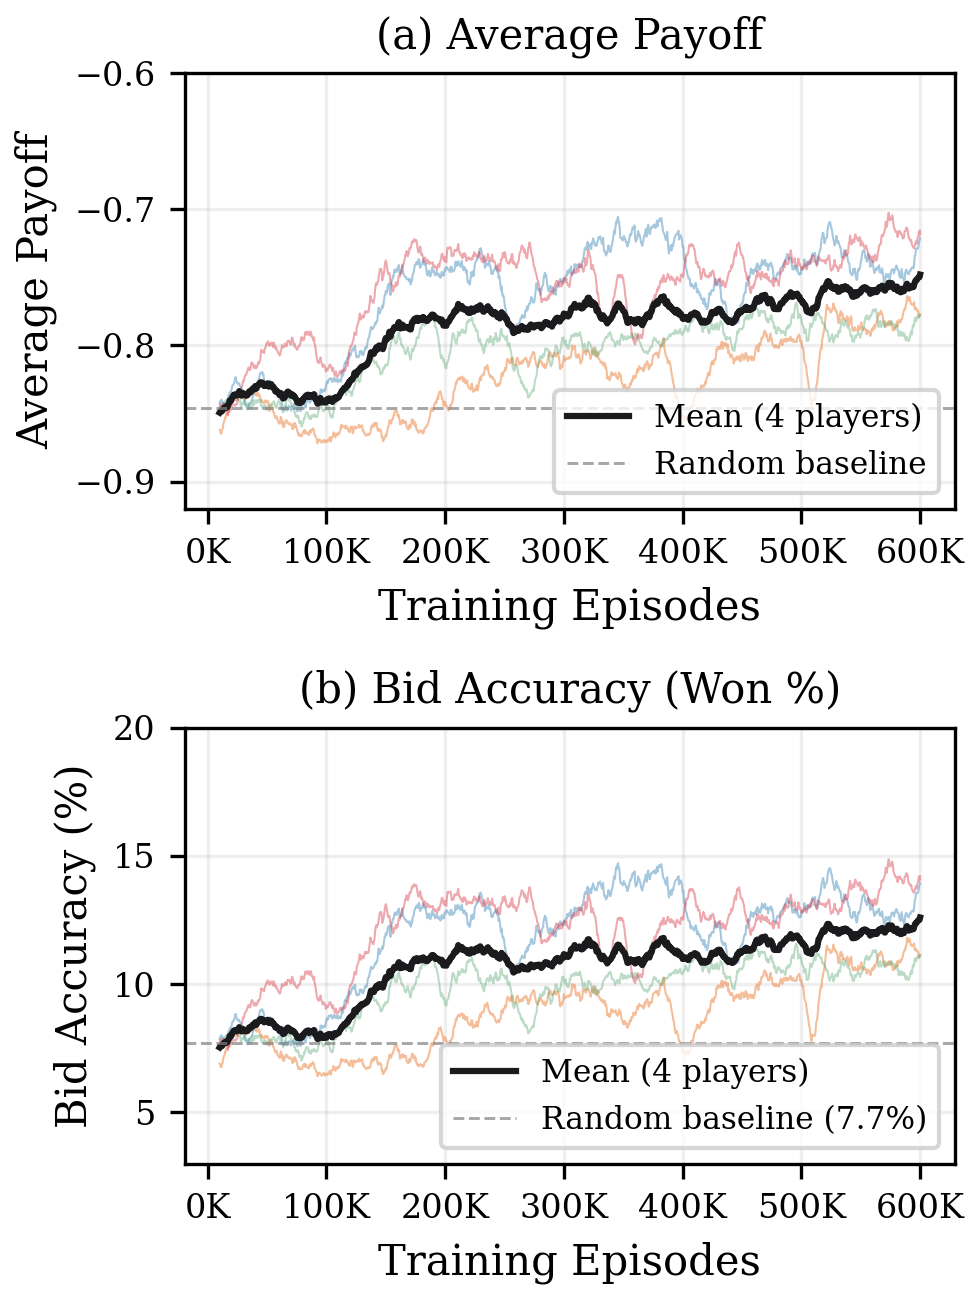
\includegraphics[width=0.85\linewidth]{training_curves.png}
\caption{Convergence of NFSP training across 600K episodes. (a) Average payoff (Averaged using 500 eval games). (b) Bid accuracy(Win$\%$). Each thin colored line represents a player, whereas the thick black line represents the mean across 4 players. The random baseline is shown by the dashed gray line.}
\label{fig:training_curves}
\end{figure}

Table~\ref{tab:milestones} tracks progress at key checkpoints in the training process. Game outcomes improve monotonically even though the loss curves behave non-monotonically, which we shall address in the Loss Dynamics subsection.

\begin{table}[!t]
\centering
\caption{\normalsize Learning Progress at Training Milestones}
\label{tab:milestones}
\scalebox{0.95}{
\small
\begin{tabular}{@{}rcccc@{}}
\toprule
\textbf{Episode} & \textbf{Avg Payoff} & \textbf{Won \%} & \textbf{RL Loss} & \textbf{SL Loss} \\
\midrule
50{,}000   & $-0.829$ & $8.5$  & $0.86$ & $0.088$ \\
100{,}000  & $-0.840$ & $8.0$  & $1.31$ & $0.139$ \\
200{,}000  & $-0.784$ & $10.8$ & $2.27$ & $0.201$ \\
400{,}000  & $-0.780$ & $11.0$ & $1.71$ & $0.105$ \\
600{,}000  & $-0.748$ & $12.6$ & $1.61$ & $0.075$ \\
\bottomrule
\end{tabular}
}
\end{table}

\subsection{\textbf{Bidding Behavior Evolution}}

Figure~\ref{fig:bidding} and Table~\ref{tab:bid_shift} reveals that under-bidding collapses from $\sim\!64\%$ early to $\sim\!20\%$ at convergence, while over-bidding rises from $\sim\!28\%$ to $\sim\!67\%$.

\begin{figure}[!t]
\centering
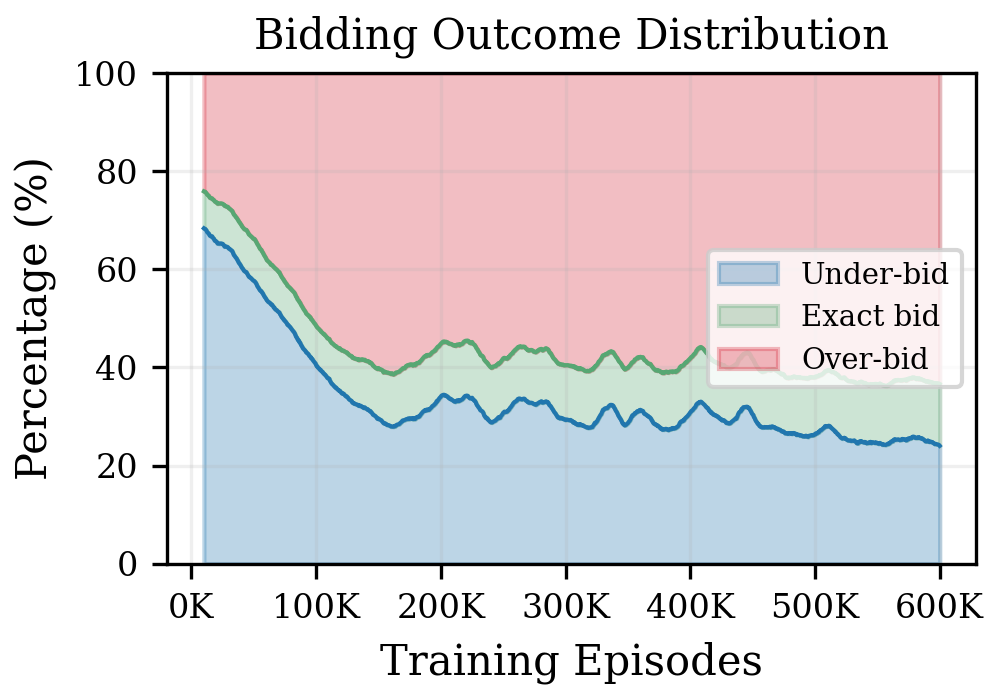
\includegraphics[width=0.85\linewidth]{bidding_evolution.png}
\caption{Evolution of bidding outcome distribution during training. (a) Under-bidding (blue) (b) Over-bidding (red) (c) Exact match (green)}
\label{fig:bidding}
\end{figure}



\begin{table}[!t]
\centering
\caption{\normalsize Bidding Behavior Shift During Training (Player 0)}
\label{tab:bid_shift}
\scalebox{0.95}{
\small
\begin{tabular}{@{}lccc@{}}
\toprule
\textbf{Phase} & \textbf{Won \%} & \textbf{Under \%} & \textbf{Over \%} \\
\midrule
Early (0--50K)       & $8.3$  & $64.3$ & $27.5$ \\
Late (540K--600K)    & $12.3$ & $20.4$ & $67.3$ \\
\midrule
$\Delta$             & $+4.0$ & $-43.9$ & $+39.8$ \\
\bottomrule
\end{tabular}
}
\end{table}

Agents learn aggressive trick-winning before learning to ``duck'' i.e.deliberately lose tricks once their bid is met. Despite the asymmetric dense reward schedule, over-bidding accounts for $\sim\!67\%$ of failures at convergence.

\subsection{\textbf{Loss Dynamics}}

The RL loss peaks at $\sim\!2.4$ around episode 250K then settles to $\sim\!1.5$. The SL loss spikes at 100K--250K as the best response shifts rapidly, then decays to $\sim\!0.08$, indicating a well-calibrated average policy.

\subsection{\textbf{Player Symmetry}}

Table~\ref{tab:symmetry} shows all four seats converge within $11.2$--$12.3\%$ bid accuracy ($1.1$ pp spread). Residual differences reflect positional effects such as the Dealer's Hook constraint.

\subsection{\textbf{Prioritized Experience Replay Ablation}}
\label{sec:per}

We reran training with PER~\cite{schaul2016prioritized} (TD-error priority sampling, $\beta$: $0.4\to1.0$). As shown in Table~\ref{tab:per}, PER reduces final RL loss by $32\%$ ($1.01$ vs.\ $1.48$) and tightens player spread from $3.2$ to $1.2$ pp, but yields no significant gain in bid accuracy or payoff---confirming the bottleneck is structural rather than a sampling issue.



\begin{table}[!t]
\centering
\caption{\normalsize Final Per-Player Performance (Last 60K Episodes)}
\label{tab:symmetry}
\scalebox{0.95}{
\small
\begin{tabular}{@{}lcccc@{}}
\toprule
\textbf{Metric} & \textbf{P0} & \textbf{P1} & \textbf{P2} & \textbf{P3} \\
\midrule
Avg Payoff  & $-0.754$ & $-0.753$ & $-0.764$ & $-0.776$ \\
Won \%      & $12.3$   & $12.3$   & $11.8$   & $11.2$   \\
Under \%    & $20.4$   & $28.4$   & $28.6$   & $21.3$   \\
Over \%     & $67.3$   & $59.3$   & $59.6$   & $67.5$   \\
RL Loss     & $0.847$  & $1.495$  & $0.946$  & $0.751$  \\
SL Loss     & $0.073$  & $0.090$  & $0.075$  & $0.067$  \\
\bottomrule
\end{tabular}
}
\end{table}



\begin{table}[!t]
\centering
\caption{\normalsize PER Ablation: Final Metrics (Mean Across 4 Players, Last 60K Episodes)}
\label{tab:per}
\scalebox{0.95}{
\small
\begin{tabular}{@{}lcc@{}}
\toprule
\textbf{Metric} & \textbf{Without PER} & \textbf{With PER} \\
\midrule
Won \%              & $12.1$  & $11.9$  \\
Avg Payoff          & $-0.757$ & $-0.762$ \\
Final RL Loss       & $1.48$   & $1.01$  \\
Final SL Loss       & $0.082$  & $0.076$ \\
Player Spread       & $3.2$ pp & $1.2$ pp \\
Peak Won \% (P0)    & $18.8$   & $17.4$  \\
\bottomrule
\end{tabular}
}
\end{table}

From this, we conclude that the primary bottleneck in learning Judgement is not sample efficiency in the replay buffer, but rather a structural credit assignment challenge. Ducking is a core skill in Judgement, and improving the replay sampling distribution does not fundamentally change the fact that one-step bootstrapping limits the agent's ability to plan for multi-trick avoidance.


%% ============================================================
%% VII. LIMITATIONS
%% ============================================================
\section{\large \textbf{Limitations}}

A few limitations of the current work deserve mention:

\textbf{The Ducking Bottleneck:} The most persistent learning bottleneck is the agent's tendency to overbid and win more tricks than declared (accounting for $\sim\!67\%$ of failures at convergence). Despite the asymmetric penalties in our dense reward schedule, deliberate trick avoidance remains unresolved, representing the single largest barrier to higher bid accuracy.

\textbf{Simplified Round and State Representation:} NFSP training is confined to single 13-card rounds rather than the full multi-round sequence of varying hand sizes typical in competitive Judgement. Additionally, the MLP network topology cannot natively exploit sequence-dependent features or temporal correlations in players' cards.

\textbf{Static Opponent Modeling and Determinization:} The PANES agent models opponents using aggregate equilibrium average policies ($\pi_{\text{avg}}$) rather than dynamically updating beliefs based on in-context play. Furthermore, the MRV determinization does not maintain a probabilistic posterior over hidden opponent cards, reducing MCTS simulation accuracy in high-uncertainty early rounds.

%% ============================================================
%% VIII. FUTURE WORK
%% ============================================================
\section{\large \textbf{Future Work}}

This work opens several directions for future research:

\textbf{Hierarchical and Adaptive Rewards:} To resolve the ducking bottleneck, future work will explore hierarchical RL architectures that switch between aggressive trick accumulation and defensive avoidance policies once the bid is met, alongside non-linear penalty scaling for over-winning.

\textbf{Attention-Based Sequence Architectures:} Swapping the MLP for Transformer-based architectures will allow dynamic attention over trick histories and seat order, facilitating void inference. Furthermore, extending self-play training across variable hand sizes (1 to 13 cards) will enable learning of round-dependent bidding strategies.

\textbf{Bayesian Opponent Modeling and Human Play:} Integrating particle filters to maintain a probabilistic belief distribution over opponent hands during online search should increase determinization accuracy. Finally, conducting user studies comparing human players against PANES will provide a benchmark for real-world play.

%% ============================================================
%% IX. CONCLUSION
%% ============================================================
\section{\large \textbf{Conclusion}}

This paper introduced PANES, a reinforcement learning framework for the trick-taking game Judgement. By integrating Neural Fictitious Self-Play (NFSP) with Information Set MCTS, PANES addresses the challenges of high non-stationarity, long credit assignment horizons, and vast information asymmetry. Our custom environment models the full complexity of Judgement under realistic rules and Hook constraints.

In self-play, agents successfully transition from simple trick accumulation to exact contract matching, though defensive ducking remains a key challenge. In arena tournaments, wrapping the trained networks in our asymmetric MCTS search shell yields a $22.7\%$ bid accuracy compared to $13.5\%$ for pure NFSP—representing a $68\%$ relative improvement ($p < 0.0001$). This advantage is consistent across all seats, demonstrating that combining offline equilibrium learning with online tree search is an effective approach for imperfect information card games.

%% ============================================================
%% REFERENCES
%% ============================================================
\bibliographystyle{IEEEtran}
\bibliography{references}

\end{document}
